\documentclass{beamer}
%\usepackage{caption}
%
%\usepackage{subcaption}
\usepackage{../arbenson-math}
\usepackage{wasysym}

\newcommand{\A}{\mathcal{A}}
\newcommand{\B}{\mathcal{B}}

\usetheme{boxes}
\usecolortheme{seahorse}

\usepackage[lined]{algorithm2e}

\setbeamertemplate{frametitle}
{
    \nointerlineskip
    \begin{beamercolorbox}[sep=0.3cm,ht=1.8em,wd=\paperwidth]{frametitle}
        \vbox{}\vskip-2ex%
        \strut\insertframetitle\strut \hfill \insertframenumber
        \vskip-0.8ex%
    \end{beamercolorbox}
}

\AtBeginSection[]
{
  \begin{frame}<beamer>
    \frametitle{\insertsection}
    \tableofcontents[currentsection]
  \end{frame}
}

\titlegraphic{}

\title{Silent error resilience \\
in numerical time-stepping schemes}
\author{
Austin Benson* \\
Institute for Computational and Mathematical Engineering \\
Stanford University \\
\vspace{0.1in}
Sven Schmit* (ICME) and Rob Schreiber (HP Labs) \\
\vspace{0.2in}
SIAM PP 2014 \\
\vspace{0.2in}
* work done while interning at HP Labs
}
\date{February 19, 2014}
\begin{document}
\maketitle

%
\begin{frame}
\frametitle{Illustrative example}

\begin{figure}
  \centering
  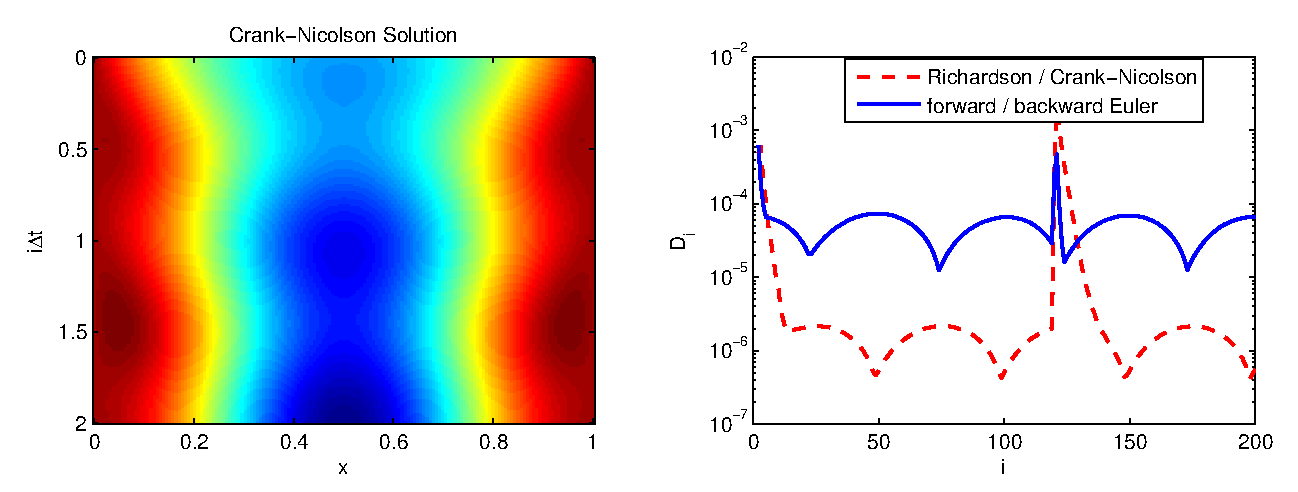
\includegraphics[scale=0.5]{figs/heat_soln_diffs1.eps}
  \vspace{-1cm}
\end{figure}

\begin{align}
& u_t = \frac{1}{100}u_{xx} + 0.1\left(\sin(2\pi t) + \cos(2\pi x)\right) \nonumber \\
& t \in [0, 2], x \in [0, 1] \nonumber \\
& u(x, 0) = x(x-1) \nonumber \\
& \Delta x = 1 / 160, \Delta t = 1 / 100 \nonumber 
\end{align}

\end{frame}

\begin{frame}
\frametitle{Illustrative example: what's at fault?}

\begin{figure}
  \centering
  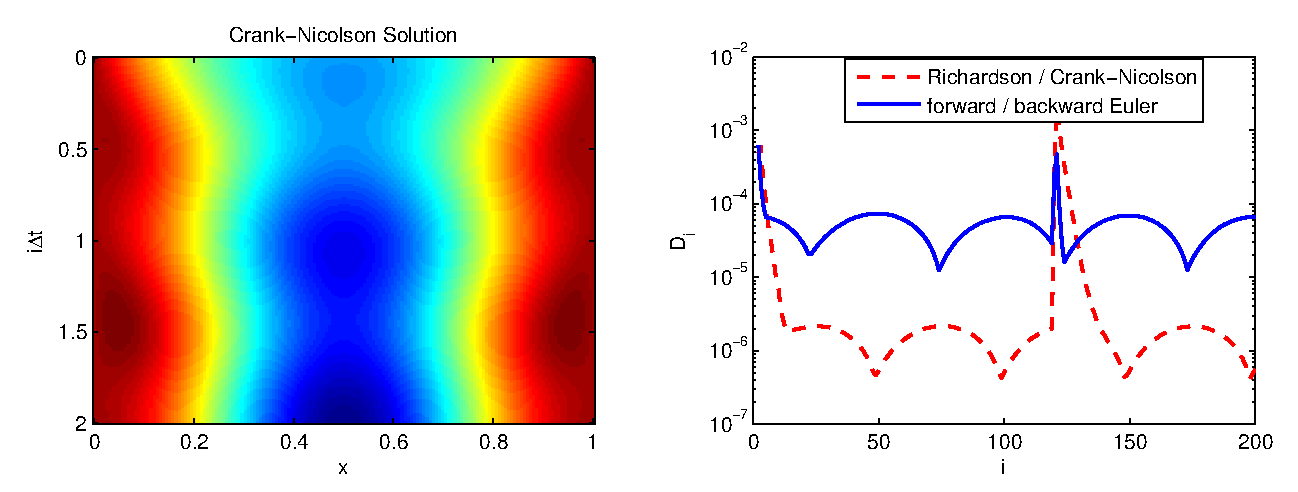
\includegraphics[scale=0.5]{figs/heat_soln_diffs1.eps}
\end{figure}

\begin{itemize}
\item At step 120, multiplied \emph{single entry} in RHS of Crank-Nicolson and Backward Euler linear solves by 0.995
\end{itemize}

\end{frame}

%
\begin{frame}
\frametitle{Main idea}

\begin{figure}
  \centering
  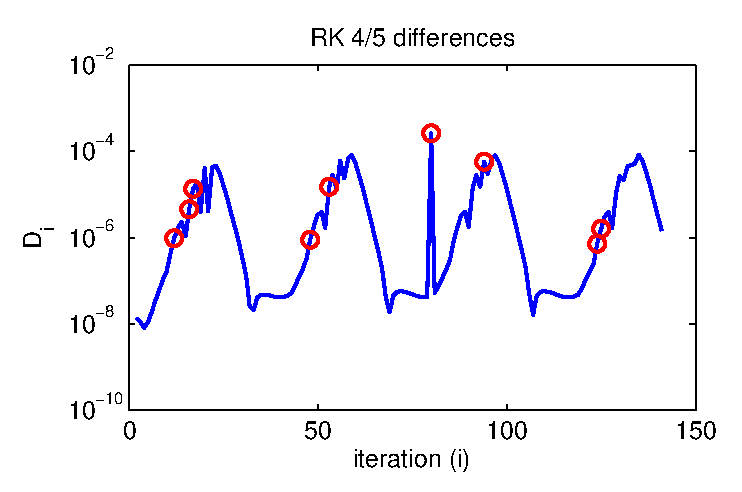
\includegraphics[scale=0.5]{figs/vdp2_rk.eps}
\end{figure}

\begin{itemize}
\setlength{\itemsep}{0.05in}
\item{At each time step, base method $\B$ generates $B_1, B_2, \ldots$}
\pause
\item{Auxiliary method $\A$ ``checks'' with $A_1, A_2, \ldots$}
\pause
\item{$D_i = ||B_i - A_i||$ abnormal $\to$ possible error}
\end{itemize}
\end{frame}

%
\begin{frame}
\frametitle{What are these things?}

\begin{figure}
  \centering
  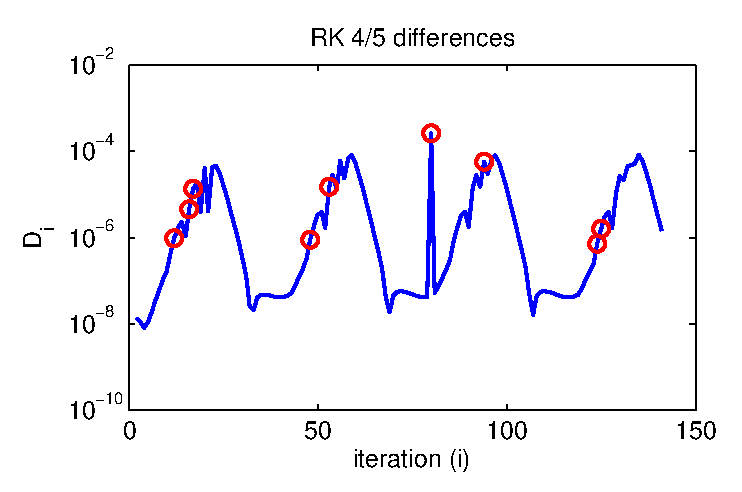
\includegraphics[scale=0.5]{figs/vdp2_rk.eps}
\end{figure}

\begin{itemize}
\setlength{\itemsep}{0.05in}
\item{Base method $\B$: higher-order scheme (Runge-Kutta 5)}
\pause
\item{Auxiliary method $\A$ ``checks'': lower-order scheme (Runge-Kutta 4)}
\pause
\item{Want $\A$ needs to be cheap: embedded pairs}
\end{itemize}

[Fehlberg, 1969],
[Dormand and Prince, 1980]

\end{frame}



%
\begin{frame}
\frametitle{Lots of these schemes}

\begin{itemize}
\item Backward / Forward Euler, Richardson / Crank-Nicolson
\item Runge-Kutta 4/5, 2/3
\item Adams-Bashforth 4/5, 2/3
\item Explicit check on implicit scheme
\item Extrapolation
\end{itemize}

\pause
\begin{itemize}
\item \textcolor{blue}{Key idea:}  Auxiliary method $\A$ re-uses data and communication from base method $\B$
\end{itemize}

\end{frame}

%
\begin{frame}
\frametitle{Detecting errors}

\begin{figure}
  \centering
  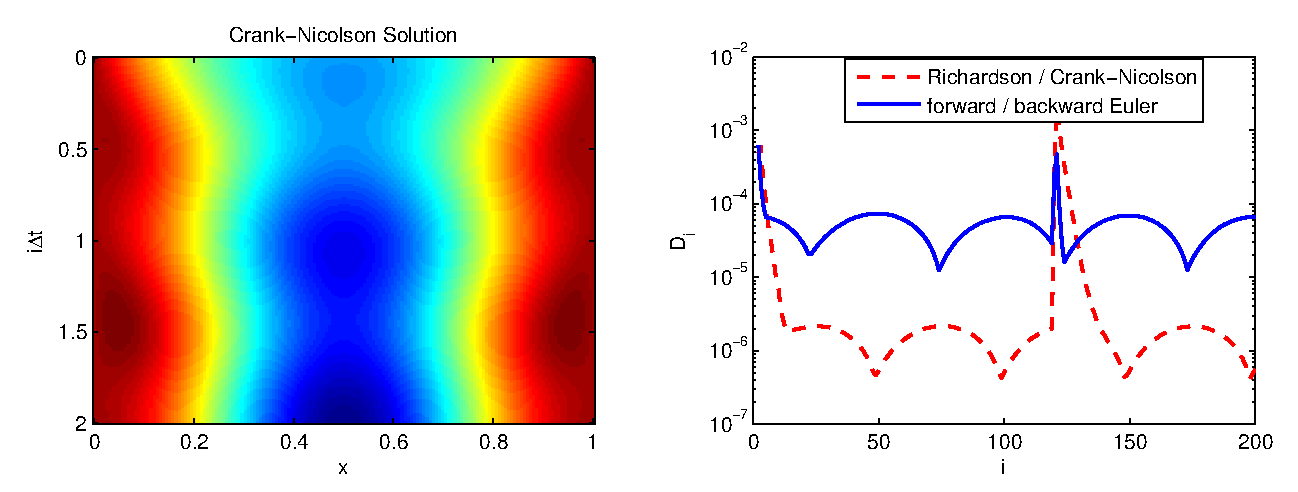
\includegraphics[scale=0.5]{figs/heat_soln_diffs1.eps}
\end{figure}

\begin{itemize}
\item Exercise in \emph{step detection}
\end{itemize}

\end{frame}

\begin{frame}
\frametitle{Detecting errors}

\begin{figure}
  \centering
  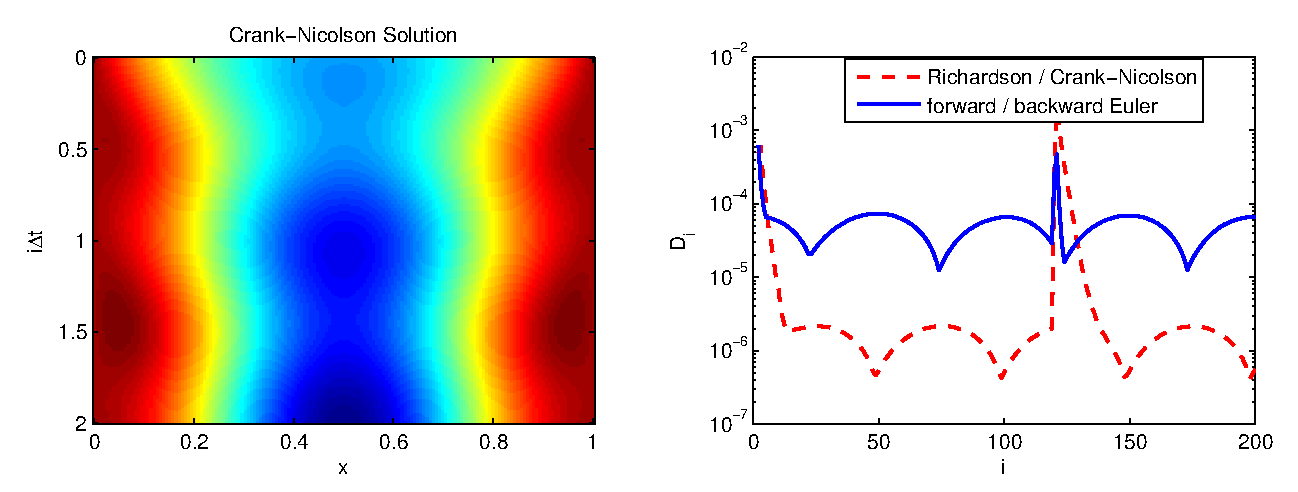
\includegraphics[scale=0.5]{figs/heat_soln_diffs1.eps}
  \vspace{-1cm}
\end{figure}


\begin{align}
& D_{n+1} = \| A_{n+1} - B_{n+1} \| \nonumber \\
& J_{n} = \frac{D_{n+1} - D_n}{D_n}, \quad \text{relative jump} \nonumber \\
& V_{n+1} = \frac{\text{Var}(D_{n-p+1}, \ldots, D_{n+1})}{\text{Var}(D_{n-p}, \ldots, D_{n})}, \quad \text{variance change} \nonumber
\end{align}

\begin{itemize}
\item $p = 4$ is usually good
\end{itemize}


\end{frame}

\begin{frame}
  \frametitle{Error detection algorithm}
  

  \begin{algorithm}[H]
  \SetKwInOut{Input}{input}
  \SetKwInOut{Output}{output}
    \Input{tolerances $\tau_J$ and $\tau_V$, scaling parameters $\Gamma > 1$, $\gamma < 1$}
      \For{$n = 1, 2, \ldots$}{
          $D_{n+1} := \| A_{n+1} - B_{n+1} \|$ \\
           \If{$J_{n+1} > \tau_J$ and $V_{n+1} > \tau_V$}{
                \texttt{FlagError()} \\
                \texttt{Move back in time} \\
           }
      }
     \lIf{$J_{n+1} > \tau_J$}{
        $\tau_J := \Gamma\tau_J$
     }\lElse{
        $\tau_J := \gamma\tau_J$     
     } \\
     \lIf{$V_{n+1} > \tau_V$}{
        $\tau_V := \Gamma\tau_V$
     }\lElse{
        $\tau_V := \gamma\tau_V$     
     }     
  \end{algorithm}
  
  \vspace{0.5cm}
  
  \begin{itemize}
    \item $\Gamma = 1.4$, $\gamma = 0.95$
  \end{itemize}
\end{frame}   


%
\begin{frame}
\frametitle{Which errors matter?}

\begin{itemize}
\item $B_n$ and $A_n$ are the outputs of $\B$ and $\A$ when \emph{a fault is injected}
\item $\hat{B}_n$ and $\hat{A}_n$ are the outputs  when \emph{no fault is injected}
\end{itemize}

\begin{center}
Local truncation error-normalized error:
\[
L_n = \frac{\| B_n - \hat{B}_n \|}{\| \hat{B}_n - \hat{A}_n \|} \approx \frac{\text{Difference caused by error}}{\text{local truncation error}}
\]
\end{center}

\end{frame}

%
%\begin{frame}
%\frametitle{Detecting errors in Adams-Bashforth}
%
%\[
%u^{\prime\prime}(t) - b(1 - u(t)^2)u^{\prime}(t) + u(t) = 0
%\]
%\[
%u(0) = 1, \quad u'(0) = 0, \quad t \in [0, T] = [0, 14]
%\]
%
%\end{frame}
%
%%
%\begin{frame}
%\frametitle{Detecting errors in Runge-Kutta}
%
%\[
%u^{\prime\prime}(t) - b(1 - u(t)^2)u^{\prime}(t) + u(t) = 0
%\]
%\[
%u(0) = 1, \quad u'(0) = 0, \quad t \in [0, T] = [0, 14]
%\]
%
%\end{frame}


%
\begin{frame}
\frametitle{Detecting errors in the heat equation}

\begin{itemize}
\item  $u_t = 0.001u_{xx} + (1 - \sqrt{1 - 4(t - t^2)}) / (2 - 2t)$
\item  $u(x, 0) = 6|x - 1/2| - 3$
\item \textcolor{red}{Error}: \\
Multiply entry of RHS in linear solves by $z \sim N(1, 5\text{e-5})$ \\
at a single time step
\end{itemize}

\vspace{-0.5cm}
\begin{figure}
  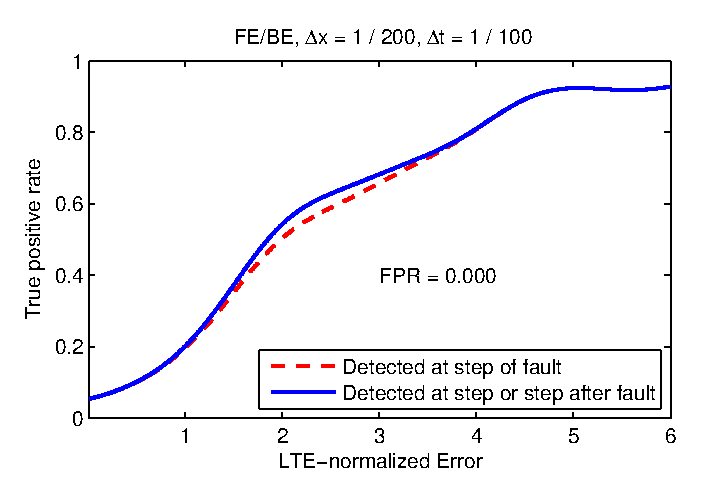
\includegraphics[scale=0.5]{figs/heat_2a_BE.eps}
  \includegraphics[scale=0.5]{figs/heat_2a_CN.eps}
\end{figure}

\end{frame}


\begin{frame}
\frametitle{Detecting errors in the heat equation}

\begin{itemize}
\item  $u_t = 0.01u_{xx} + q(x, t)$, \quad $q(x, t) = xe^{-t/2}$
\item  $u(x, 0) = 4x(x-1)(x-2)$
\item \textcolor{red}{Error}: \\
Multiply $q(x, t)$ at one discrete $x$ by $z \sim N(1, 0.1)$ \\
at a single time step
\end{itemize}

\vspace{-0.5cm}
\begin{figure}
  \includegraphics[scale=0.5]{figs/heat_1a_BE.eps}
  \includegraphics[scale=0.5]{figs/heat_1a_CN.eps}
\end{figure}

\end{frame}

\begin{frame}
\frametitle{Adams-Bashforth}

\begin{itemize}
\item $u^{''}(t) - b(1 - u(t)^2)u'(t) + u(t) = 0$
\item $u'(0) = 1$, $u(0) = 0$
\item \textcolor{red}{Error}: \\
Multiply one derivative evaluation by $z \sim N(1, 0.1)$
\end{itemize}

\begin{figure}
  \includegraphics[scale=0.6]{figs/ab23_vdp_2_func.eps}
  \includegraphics[scale=0.6]{figs/ab45_vdp_2_func.eps}
\end{figure}

\end{frame}


\begin{frame}
\frametitle{Runge-Kutta}

\begin{itemize}
\item $u^{''}(t) - b(1 - u(t)^2)u'(t) + u(t) = 0$
\item $u'(0) = 1$, $u(0) = 0$
\item \textcolor{red}{Error}: \\
Multiply one derivative evaluation by $z \sim N(1, 0.1)$
\end{itemize}

\begin{figure}
  \includegraphics[scale=0.6]{figs/rk23_vdp_2_func.eps}
  \includegraphics[scale=0.6]{figs/rk45_vdp_2_func.eps}
\end{figure}

\end{frame}


\begin{frame}
\frametitle{Tardy error detection}

\begin{figure}
  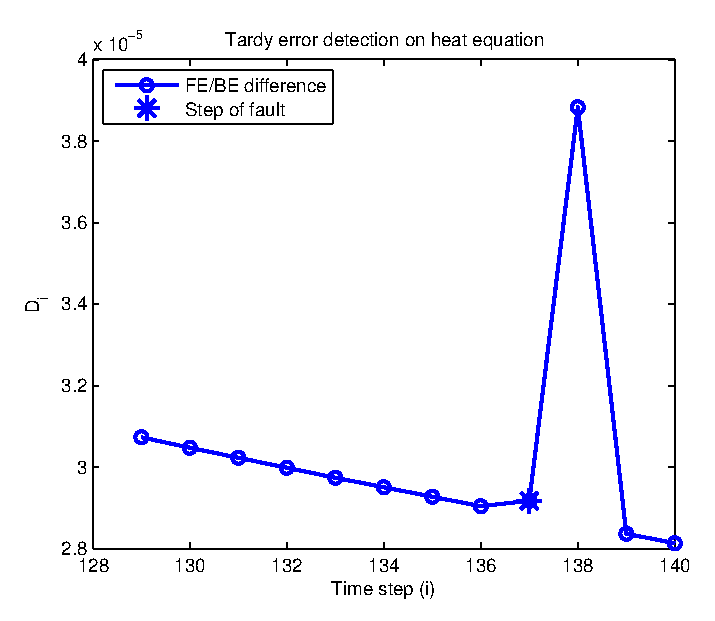
\includegraphics[scale=0.5]{figs/tardy_detection.eps}
  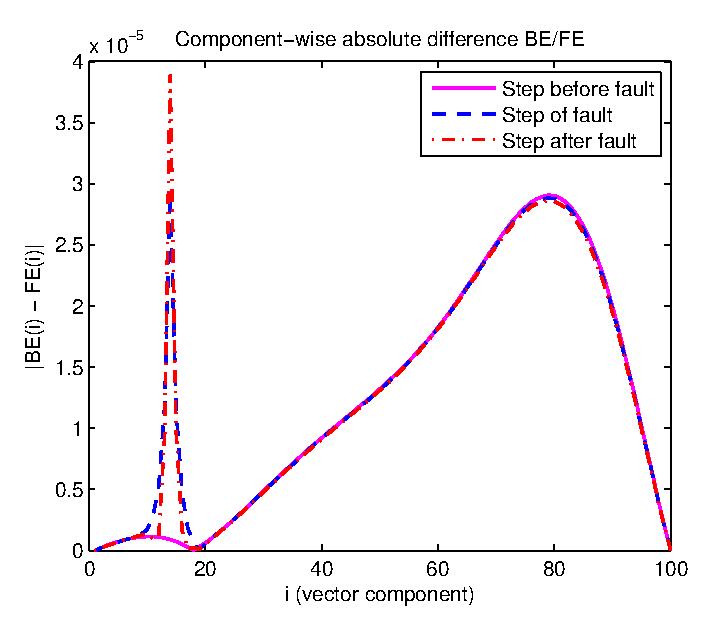
\includegraphics[scale=0.5]{figs/tardy_detection_soln.eps}
\end{figure}

\end{frame}

\begin{frame}
\frametitle{Key ideas}

\textcolor{blue}{Key ideas}:
\begin{itemize}
\item Take advantage of ``paired" solvers to check solutions
\item High-impact error $\to$ easier to detect
\item Simple detection scheme work pretty well
\end{itemize}

\end{frame}

%
\begin{frame}
\frametitle{End}

\begin{itemize}
\item Austin Benson: arbenson@stanford.edu
\item Pre-print + code + data: \url{http://stanford.edu/~arbenson}
\end{itemize}
\end{frame}

\end{document}
